\documentclass[hyperref={pdfpagelabels=false}]{beamer}
\usepackage{graphicx,lmodern,subfigure,ulem,color,graphicx,tikz,booktabs,natbib}
\usepackage{mathrsfs}
\usetheme{Warsaw}
%\definecolor{beamer@blendedblue}{rgb}{0.1,0.5,0.1}
%\definecolor{ForestGreen}{RGB}{60, 140, 60}
%\setbeamercolor{structure}{fg=beamer@blendedblue}
\setbeamertemplate{navigation symbols}{}
\setbeamertemplate{footline}[frame number]
\bibliographystyle{chicago}
\newcommand{\spitem}{\vspace{.3cm}\item}
\newcommand{\elas}{$E_{labor}$}
%\def \FigPath {Users\th3\Documents\Job_Market_Paper\Code\Figures} 


\title{Research Proposal}
\author{Marco Brianti}
\institute{Boston College}
\date{September 2018}


\begin{document}
	
	\frame{\titlepage \begin{center} Dissertation Workshop \end{center} }
	
	
		\frame{\frametitle{Relevance}
		
		\begin{center}
			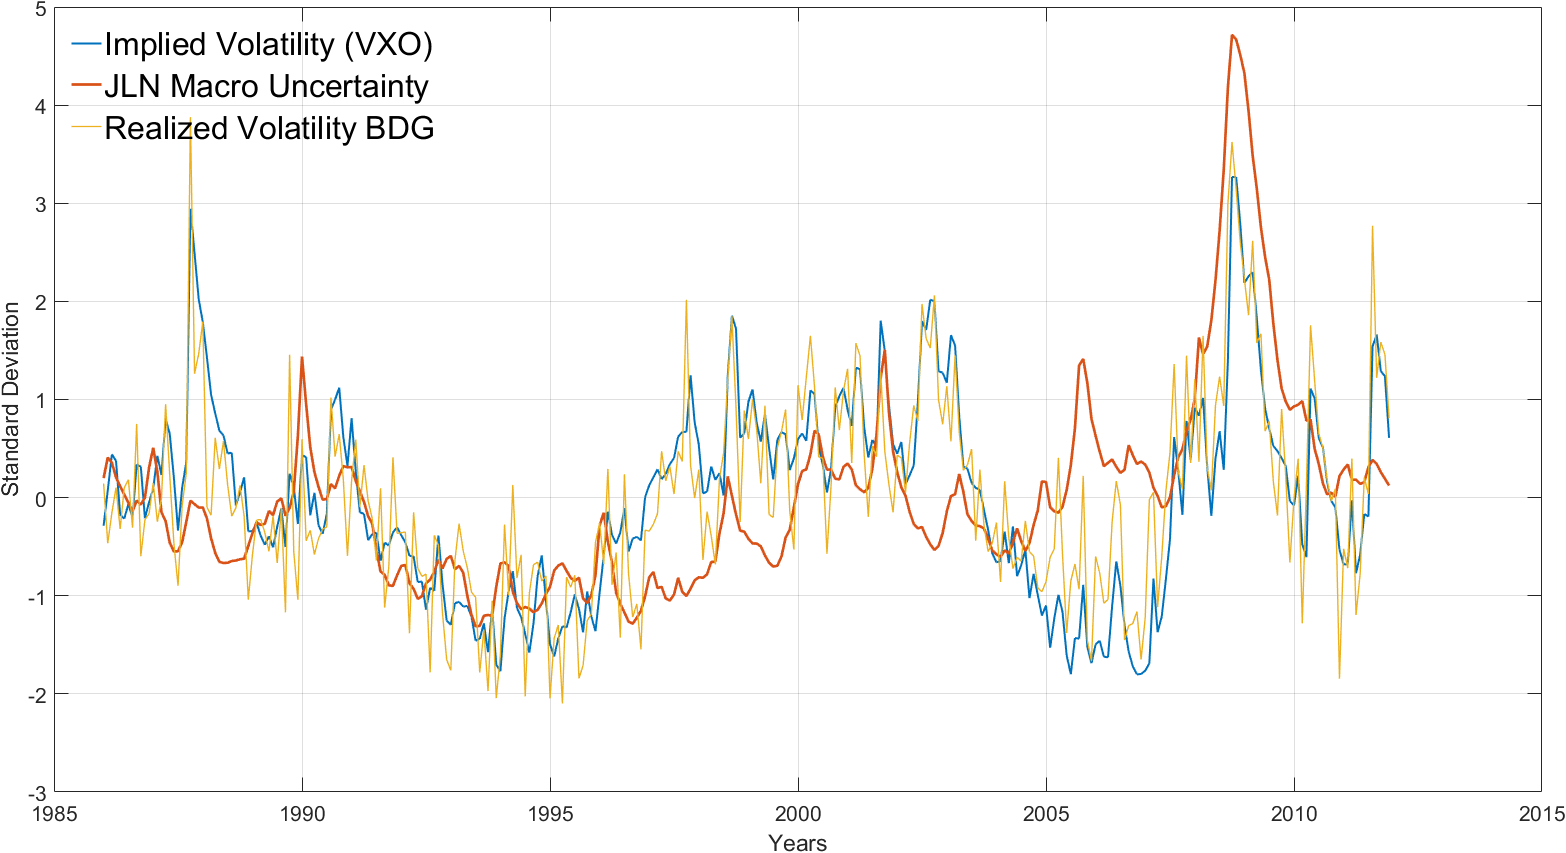
\includegraphics[scale=0.26]{Uncertainty}
		\end{center}
		
		
		\begin{center}
			\begin{tabular}{ c | c c c c}
				& VXO & JLN & BDG \\ \hline
				IP  &     -0.2358         & -0.4935         &  -0.2822    \\

			\end{tabular}
		\end{center}
		
		
	}
	
		\frame{\frametitle{Uncertainty as a driver of the business cycle}
		
		The acute instability that featured financial markets during the 2007-09 crisis and the relation with its unprecedented severity and duration have set doubts on known sources of economic fluctuations.
		
		\
		
		Since then, uncertainty has been proposed as a new potential driver of the business cycle.
		
		\
		
		Empirical literature has been called to answer the following positive questions
		
		\begin{itemize}
			\item Is uncertainty just an endogenous response to 1st-moment shocks?
			\item Does uncertainty plays an autonomous and active role as a driver of the cycle?
		\end{itemize}
		
		
	}
	
	\frame{\frametitle{Uncertainty as a theoretical concept}		
		
		\begin{itemize}
			
			\item Frank Knight in 1921 defined \textbf{uncertainty} as people's inability to forecast the likelihood of events happening.
			
			\
			
			\
		    
		    \
		    
		    \
		    
		    \item Today, uncertainty is represented by the expected volatility of the unforecastable part of key macroeconomic variables.
		    
		    \begin{itemize}
		    	\item Uncertainty $\neq$ Volatility (!)
		    \end{itemize}
		
		\end{itemize}			
}

	\frame{\frametitle{Uncertainty as an empirical measure}
	
	
\begin{itemize}
	
	\item Uncertainty cannot be directly observed
	
	\
	
	\
	
	\item A series of different proxies
	\begin{enumerate}
		\item Financial realized volatility 
		\item Financial implied (expected) volatility 
		\item Disagreement among a group of forecasters 
		\item Cross sectional dispersion of firm profits
		\item Narrative approach
	\end{enumerate}
	
	\
	
	\
	
	\item Jurado et al. (2015) provided a generalized measure of macro uncertainty which is consistent with its theoretical concept.
	
	
\end{itemize}

}	

\frame{\frametitle{Research Question}
	
	\begin{itemize}
	
\item Which is the \textbf{causal effect} of uncertainty on economic activity?	

\

\

\item In other words, which is the effect of an \textbf{uncertainty shock} on macroeconomic variables?

\

\

\item Ideally, I would like to estimate through a \textbf{semi-structural model} a series of \textit{primitive} and \textit{exogenous} changes in agents' ability to forecast economic variables.

\begin{itemize}
\item In this specific case, structural models tend to impose the result by construction. 
\end{itemize}
	
	\end{itemize}
	
}

	
	\frame{\frametitle{Main Contribution}
		
		\begin{enumerate}
			\item Provide a new empirical evidence on the effect of uncertainty shocks 
			
			\
			
			\item Show how to clean out uncertainty shocks from signals regarding future states of the economy
			
			\
			
			\item Suggest a new family of internal instruments able to disentangle financial shocks from uncertainty shocks
		\end{enumerate}
		
		
		
	}



	\frame{\frametitle{Main Related Literature}
		


			\begin{itemize}
				\item Stock and Watson (2012) - Brookings;
				\item Jurado, Ludvigson, and Ng (2015) - AER;
				\item Caldara, Fuentes-Albero, Gilchrist, and Zakrajsek (2016) - EER;
				\item Berger, Dew-Becker, and Giglio (2019) - R\&R REStud;
				\item Cascaldi-Garcia and Galvao (2019) - forthcoming JMCB;
				\item Ludvigson, Ma, and Ng (2017) - NBER working paper. 
				\item Carriero, Clark, and Marcellino (2019) - forthcoming REStat
				\item Carriero, Clark, and Marcellino (2018) - working paper
			\end{itemize}    
	
		
	}

	\frame{\frametitle{Challenges}
		
		\begin{enumerate}
			\item It is a \textbf{latent variable}
						\begin{itemize}
				\item it cannot be directly observed
			\end{itemize}
		
		\
			
			\item Potential \textbf{simultaneity} with other shocks
			\begin{itemize}
				\item uncertainty responds on impact to any 1st-moment shocks
				\item aggregate variables respond on impact to uncertainty shocks
			\end{itemize}
		
		\
		
		\item Potential \textbf{reverse causality} with any news shocks
					\begin{itemize}
			\item Signal regarding future states of the economy may affect current uncertainty 
		\end{itemize} 
	

\

\item It is deeply confounded with \textbf{financial shocks}
\begin{itemize}
	\item Exogenous changes in borrowing conditions
\end{itemize}
	
	
		\end{enumerate}
		
	}

	\frame{\frametitle{Technically Speaking (I)}
		
		Assume you use OLS techniques to regress $X_t$ on its own past
		$$
		X_t = B_1 X_{t-1} + B_2 X_{t-2} + \dots + B_p X_{t-p} + \iota_t
		$$
		where $X_t = [U_t \ \  Y_t  \ \  F_t]'$, $U_t$ represents a proxy for uncertainty, $Y_t$ a column vector of macro variables, and $F_t$ a vector of financial variables.
		
		\
		
		Moreover, $\iota_t = [\iota^U_t \ \ \iota^Y_t \ \ \iota^F_t]'$ is a vector of time-varying innovations related to the corresponding variables.
		
		\
		
		In general, $\iota_t$ does not represent a vector of structural shocks since 
		$$
		\iota_t \iota_t' \neq I_n
		$$
		which implies that innovations represent a (linear) combination of the structural shocks.
	}

	\frame{\frametitle{Technically Speaking (II)}
	
	
	Structural VARs methods aim to solve the following system in order to recover structural shocks
	$$
	\iota_t = C s_t \ \ \Rightarrow \ \ s_t = C^{-1} \iota_t \ \ \Rightarrow \ \ s_t = A \iota_t
	$$
	which is
	$$
    \begin{cases}
	s_t^U = A_{11} \iota_t^U + A_{12} \iota_t^Y + A_{13} \iota_t^F \\
	s_t^Y = A_{21} \iota_t^U + A_{22} \iota_t^Y + A_{23} \iota_t^F \\
	s_t^U = A_{31} \iota_t^U + A_{32} \iota_t^Y + A_{33} \iota_t^F
	\end{cases}
$$

\begin{enumerate}
	\item \textbf{Latent variable} $\Rightarrow$ $\iota_t^U$ may not represent innovations to uncertainty
	
	
	\item \textbf{Simultaneity} $\Rightarrow$ Each element of $A$ is different from zero
	
	\item \textbf{Reverse causality} $\Rightarrow$ $\iota_t^U$ may be lead by $s_{t,t+h}$, $h > 0$
	
	
	\item \textbf{Financial shocks} $\Rightarrow$ $E [ \iota_t^U  \iota_t^{F'}]  \neq 0$ and large
	
\end{enumerate}

}


	\frame{\frametitle{(1) Latent Variable}
		
		Not surprisingly, $Corr(VXO_t, JLN_t) = 0.4139$
		
		\
		
		However, $Corr(\iota_t^{VXO},\iota_t^{JLN}) \in [-0.1865 \ \ 0]$
	
\

Which means that although the 2 raw series are highly correlated, once we control for available information at $t-1$ then they convey different information.

\

\textbf{Solution.} JLN proxy is consistent with the theoretical definition of uncertainty. 

\

$\Rightarrow$ VXO measures \textbf{macro volatility} and not macro uncertainty.

	
}




	\frame{\frametitle{(2) Simultaneity with other shocks}

	
In general,	
$$
corr(\iota^{JLN}_t,s^Y_t) \approx 0
$$
which implies that uncertainty innovations are fairly uncorrelated with macro structural shocks series derived in the literature.

\

$s_t^Y$ are several series of macro structural shocks derived by the literature (possibly via narrative approach). 
\begin{itemize}
	\item Romer and Romer (2010) unanticipated tax shocks
	\item Martens and Ravn (2011) labor productivity shocks
	\item Leeper et al. (2013) anticipated tax shocks
	\item Kilian (2009) oil shocks
	\item \dots
\end{itemize}
}


	\frame{\frametitle{(3) Reverse causality with news shocks}
		
		\begin{itemize}
			
			\item \textbf{JLN proxy} controls for the forecastable part of each variable
			
			\
			
			
			\item Some structural shocks shown above are \textbf{anticipated}
			
			\
			
			
			\item We can possibly control for \textbf{news shocks} to TFP
			\begin{itemize}
				\item However, we will have to assume that TFP is fully exogenous
			\end{itemize}
			
			\
			
			
			\item \textbf{Surveys} can help for the short run horizon
			\begin{itemize}
				\item SPF has the best timing
			\end{itemize}
		
		\
		
		
			\item Most importantly, we should control for the shocks and the \textbf{square of the shocks}
			\begin{itemize}
				\item Potentially, uncertainty may evenly react for large shocks no matter the sign
			\end{itemize}
		
		
		\end{itemize}
	
}

	\frame{\frametitle{(4) Financial Shocks vs Uncertainty Shocks}
	
Stock and Watson (2012); Caldara, Fuentes-Albero, Gilchrist, and Zakrajzek (2016) shown that uncertainty shocks and financial shocks are deeply confounded.
$$
corr(\iota^{EBP}_t,\iota^{JLN}_t) \approx 0.45
$$
where $\iota^{EBP}_t$ is an innovation in the \textbf{excess bond premium} from Gilchrist and Zakrajzek (2012).

\

\

Literature did not succeed yet to disentangle the two exogenous sources:
\begin{itemize}
	\item \textbf{External instruments} do not seem to be available
	\item \textbf{Internal instruments} are difficult to find because variables respond analogously to both shocks
\end{itemize}
	
}



	\frame{\frametitle{(4) Financial Shocks vs Uncertainty Shocks - Solution (I)}
		
I propose a \textbf{novel family of internal instruments} which can help out to disentangle the two exogenous shocks.	

\

\textbf{Economic Intuition.} 

\begin{itemize}
	\item An exogenous deterioration of credit conditions should display the attempt of borrowers to fund their projects with \textbf{alternative sources} (at least on impact): internal cash flow, equity issuance, ...
	\item Alternatively, following real-options models (Bernanke, 1983; Brennan and Schwartz, 1985; McDonald and Siegel, 1986) after an uncertainty shock firms prefer to \textbf{wait-and-see} without undertake any investment.
\end{itemize}

	
	}


	\frame{\frametitle{(4) Financial Shocks vs Uncertainty Shocks - Solution (II)}
	
	Although the impact effect on investment is expected to be negative in both cases, I expect
	\begin{itemize}
		\item a financial shock to have a \textbf{negative impact} on internal cash flow;
		\item an uncertainty shock to have a \textbf{non-negative impact} on internal cash flow.
	\end{itemize}

\

\
	
The two shocks can be disentangled via \textbf{sign restrictions} \`a la Uhlig (2005)
	
	
}


\end{document}